\documentclass[10pt]{article}
\usepackage[margin=0.78in]{geometry}
\usepackage{booktabs}
\usepackage{amsmath}
\usepackage{array}
\usepackage{graphicx}
\usepackage{microtype}
\usepackage{xcolor}
\usepackage[hidelinks]{hyperref}

\newcommand{\ncd}{\textsc{NCD}}
\newcommand{\mean}[1]{\overline{#1}}

\title{Measuring Silent Explanation Drift in Task-Free\\
Class-Incremental Network Intrusion Detection}
\author{Research draft}
\date{Evidence freeze: 11 October 2026 (complete Phase-I Exp.~3 matrix)}

\begin{document}
\maketitle

\begin{abstract}
Predictive accuracy and catastrophic forgetting do not reveal whether a
continually learned intrusion detector preserves the feature evidence behind
an otherwise stable class decision.  We study \emph{silent explanation drift}:
an adjacent-checkpoint change in class-level feature attribution while class
recall drops by less than five percentage points.  Our audit repeats three
direct PyTorch attribution methods over fixed probes and backgrounds, compares
the conventional fixed Jaccard rule with repeat averaging, and evaluates a
noise-calibrated permutation test (\ncd) with within-run false-discovery-rate
control and cross-explainer consensus.  An intervention-grounded benchmark on
NSL-KDD and UNSW-NB15 gives \ncd{} one false positive in 104 known-negative
cases, while a repeat-mean baseline gives none; both detect all 26 eligible
strong shortcut cases and all nine eligible feature-masking cases.  Thus the
current \ncd{} mechanism does not outperform simple repeat averaging.  The
complete four-dataset, seven-learner, five-seed Phase-I matrix contains 1088
silent class--transition units.  \ncd{} labels 1076 (98.90\%) as drift, versus
695 (63.88\%) for the single-estimate rule and 692 (63.60\%) for repeat
averaging.  Its rate remains 97.33--99.54\% over registered FDR thresholds and
reaches 100\% on both CIC datasets.  High agreement therefore reflects
saturation rather than established detector validity.  These negative results
bound the contribution to an auditable measurement study and motivate
intervention-based validation before any governance or innovation claim.
\end{abstract}

\section{Introduction}

Class-incremental network intrusion detection (NIDS) is normally assessed by
final predictive performance and catastrophic forgetting.  This is necessary
but incomplete: an update may preserve a class prediction or recall while
changing the evidence used to support it.  Such a change matters when an
explanation is used for audit, analyst communication, or governance, yet a raw
difference between two stochastic explanations is not automatically a model
change.

The scientific object in this study is the predictive, retention,
explanatory, and governance behaviour of task-free class-incremental NIDS over
successive checkpoints.  The implementation, explainer, and detector are
instruments rather than the research object.  We ask three locked questions:
(RQ1) how often silent explanation drift occurs and how it varies across data,
learners, and thresholds; (RQ2) what prediction, class-safety, forgetting,
memory, and cost trade-offs the learners exhibit; and (RQ3) whether explanation
evidence can support an auditable non-suppressive governance process.  The
present paper directly addresses RQ1 and reports a bounded RQ2 measurement.
RQ3 remains unanswered by the current evidence and is not replaced by the
drift detector.

The study makes three evidence-bounded contributions.  First, it defines a
fixed-probe, adjacent-checkpoint audit of the actual class logit rather than a
surrogate backward pass.  Second, it introduces an intervention benchmark with
known negative and positive dependency changes, allowing explanation-change
rules to be evaluated as detectors.  Third, it reports a negative mechanism
result: on the completed intervention cells, simple repeat averaging matches or
outperforms the current permutation-based \ncd{} decision.  These contributions
do not establish substantive algorithmic innovation or publication readiness.

\section{Related work and exact distinction}

CLEX established explanation drift as a continual-learning problem and showed
that similar predictive performance need not imply similar explanations
\cite{cossu2024clex}.  RRR instead constrains continual training to preserve
stored explanations \cite{ebrahimi2021rrr}.  E2D2 monitors explanation
fingerprints for drift in unsupervised NIDS \cite{nugraha2026e2d2}, while
Drift2Act studies budgeted responses and online risk certification rather than
attribution-drift validity \cite{lamaakal2026drift2act}.

Estimator uncertainty is also established prior art.  Covert and Lee derive
convergence and uncertainty estimates for KernelSHAP \cite{covert2021kernel},
GPEC combines approximation uncertainty with decision-boundary complexity
\cite{hill2024gpec}, and population Shapley inference provides confidence
intervals and hypothesis tests for a global estimand
\cite{williamson2020spvim}.  Recent work on SHAP multiplicity explicitly
separates repeated-explainer randomness from model/training multiplicity and
uses randomized baselines \cite{hwang2026multiplicity}.  This is material
novelty risk.  Our narrower distinction is the conjunction of adjacent
class-incremental checkpoints, class--transition-level label permutation,
within-run FDR, cross-explainer consensus, silent-recall conditioning, and
intervention-derived truth in NIDS.  A targeted ten-source review found no
exact match, but that bounded search is not proof of novelty.

\section{Experimental design}

\subsection{Datasets and continual learners}

The registered real-data matrix contains NSL-KDD, UNSW-NB15, CIC-IDS-2017,
and CSE-CIC-IDS2018.  Task order, split, preprocessing, memory limits, and seeds
$\{1,2,3,4,42\}$ are fixed within each dataset.  The seven Phase-I learners are
Naive fine-tuning, EWC, LwF, Replay, Replay-Herding, Replay-DPMeans, and iCaRL.
Each task boundary produces a checkpoint.  The official test population is
used only for frozen post-training evaluation, not model selection.

We report accuracy on currently seen classes, balanced accuracy, macro F1,
per-class recall, Normal-class recall, and signed average forgetting.  For
class $c$, forgetting at the final checkpoint is
\begin{equation}
F_c = \max_{t<T} R_{c,t} - R_{c,T},
\end{equation}
averaged over classes observed before the final checkpoint.  Negative values
are retained rather than clipped because later performance may exceed all
earlier recorded values.

\subsection{Explanation audit}

For every checkpoint and class, the audit uses at most 200 fixed test probes
and a fixed background of 100 Task-0 training rows.  Expected Gradients,
Feature Ablation, and Gradient$\times$Input operate on the true PyTorch class
logit.  Each checkpoint generates ten explainer repetitions and ten probe
bootstraps.  Class-level mean absolute attributions are normalized to sum to
one.

For an adjacent checkpoint pair, the primary distance is one minus Spearman
rank correlation over all features.  Jaccard distances at
$k\in\{5,10,15,20\}$ are secondary.  A transition is silent at the primary
tolerance when
\begin{equation}
\Delta R_c = R_{c,t+1}-R_{c,t} > -0.05.
\end{equation}
Sensitivity is retained at tolerances $\{0,0.02,0.05,0.10\}$.

Figure~\ref{fig:ncd-architecture} separates the observational learner outputs,
fixed audit inputs, explanation measurements, calibrated decision, matched
controls, and research endpoints.  In particular, the audit never suppresses
or updates a model, and the RQ3 governance path remains downstream and
unvalidated.

\begin{figure*}[t]
  \centering
  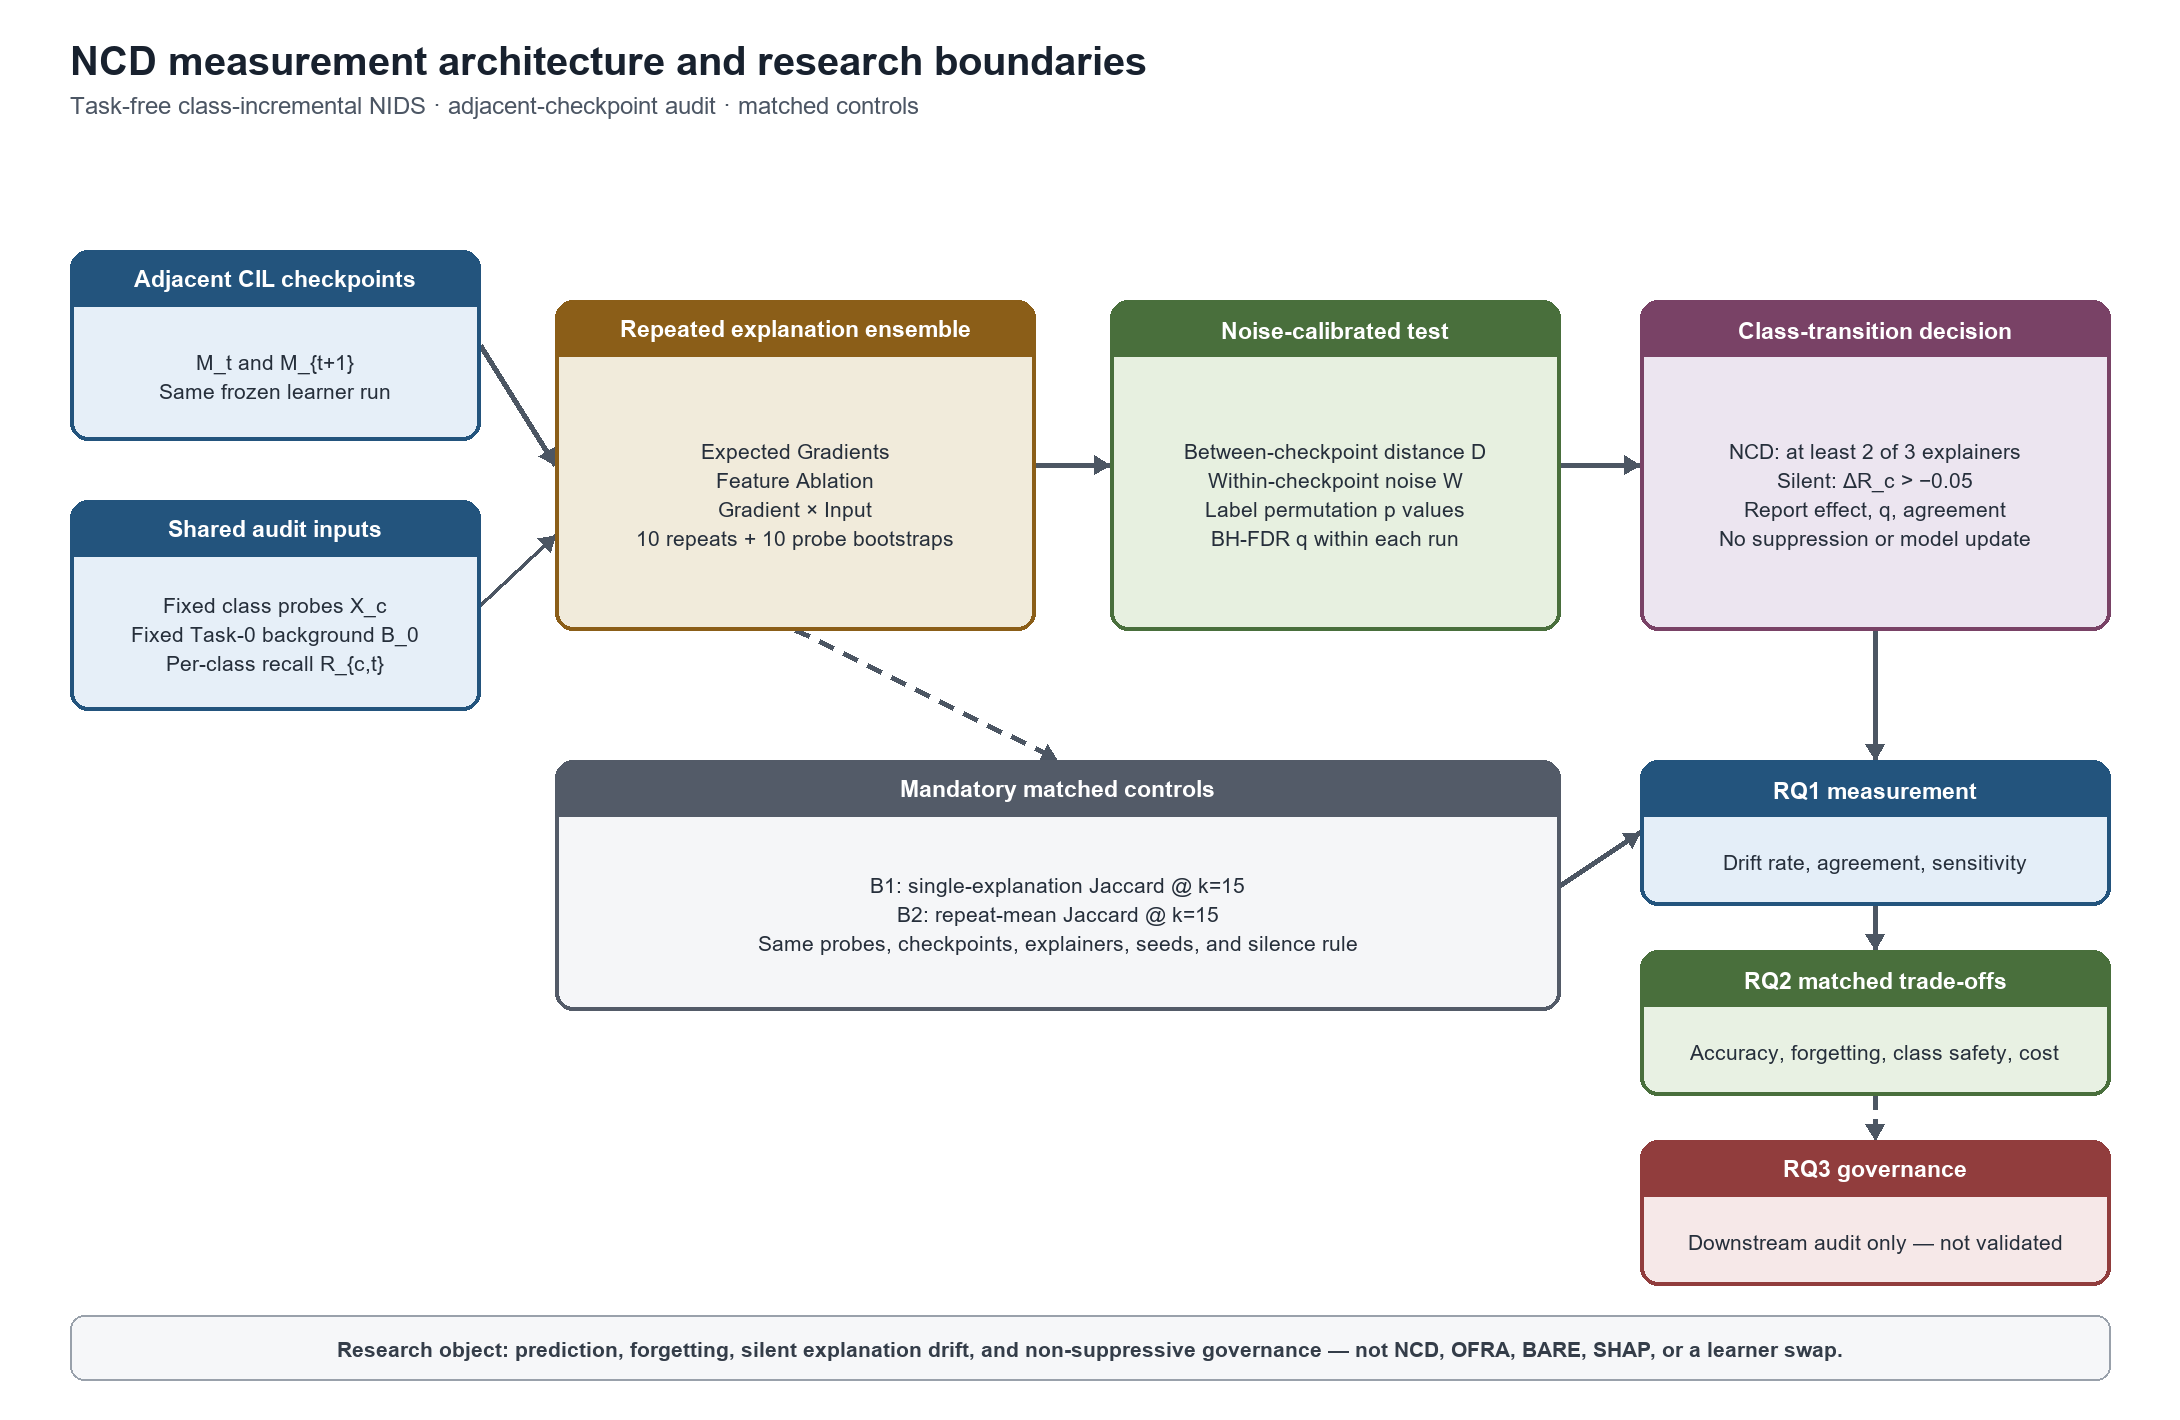
\includegraphics[width=\textwidth]{figures/ncd_method_architecture.png}
  \caption{NCD measurement architecture and research boundaries.  Frozen
  adjacent checkpoints, probes, and backgrounds feed three repeated
  explainers.  Within- versus between-checkpoint distances are tested using
  permutation and within-run FDR; at least two of three explainers must agree.
  B1 and B2 remain matched fixed-threshold controls.  NCD is a
  non-suppressive measurement mechanism, not the research object, and RQ3 is
  not validated by the current evidence.}
  \label{fig:ncd-architecture}
\end{figure*}

\subsection{Detectors}

B1 is the single-estimate rule $J@15<0.70$.  B2 applies the same threshold to
the mean of repeated attribution estimates.  For \ncd, let $D_B$ be the
between-checkpoint distances and $D_W$ the within-checkpoint distances.  The
test statistic is
\begin{equation}
T = \operatorname{median}(D_B)-\operatorname{median}(D_W).
\end{equation}
The two checkpoint labels are permuted over the pooled estimates at least 1000
times.  Benjamini--Hochberg correction is applied across all class--transition
tests inside each dataset--method--seed run at $q=0.05$.  The primary decision
requires significance from at least two of the three explainers; a Cauchy
combination is retained as a secondary analysis.

\subsection{Intervention-derived truth}

N1 re-explains the same checkpoint.  N2 applies a function-preserving hidden
unit permutation or positive ReLU scaling and verifies a maximum logit
difference below $10^{-5}$.  P1 injects a synthetic marker that becomes
class-correlated at the later task; marker permutation at test time must reduce
class accuracy by at least five percentage points to establish a positive
dependency change.  P2 masks or perturbs selected features and uses the same
interventional criterion.  Only positive constructions satisfying the silent
recall condition enter the positive detector denominator.

\section{Intervention-grounded results}

Table~\ref{tab:exp2} reports the frozen five-seed matrix.  The prespecified
point gate is met, including UNSW-NB15 iCaRL exactly at the 5\% boundary.
However, B2 detects every eligible positive detected by \ncd{} and has fewer
negative-control false positives.  With only 20--34 negative controls per
cell, the observed proportions do not establish a population FPR below 5\%.

\begin{table}[ht]
\centering
\caption{Frozen Exp.~2 detector counts.  P1 denotes strong shortcuts
($\rho\geq0.9$); P2 is unavailable when no eligible intervention was found.}
\label{tab:exp2}
\small
\begin{tabular}{llrrrrrr}
\toprule
Dataset & Learner & \multicolumn{2}{c}{Negative FP} & \multicolumn{2}{c}{P1 detected} & \multicolumn{2}{c}{P2 detected} \\
 & & \ncd & B2 & \ncd & B2 & \ncd & B2 \\
\midrule
NSL-KDD & Replay & 0/34 & 0/34 & 8/8 & 8/8 & 5/5 & 5/5 \\
UNSW-NB15 & Replay & 0/30 & 0/30 & 5/5 & 5/5 & 4/4 & 4/4 \\
NSL-KDD & iCaRL & 0/20 & 0/20 & 9/9 & 9/9 & -- & -- \\
UNSW-NB15 & iCaRL & 1/20 & 0/20 & 4/4 & 4/4 & -- & -- \\
\bottomrule
\end{tabular}
\end{table}

The independently executed 25-run NSL-KDD drift tranche covers Naive, EWC,
LwF, Replay-Herding, and Replay-DPMeans over the same five seeds.  Its matched
performance evaluation is now included in Table~\ref{tab:exp3full}.  Across 157 silent
class--transition units, B1 and B2 each flag 52 (33.12\%), whereas \ncd{} flags
154 (98.09\%).  Method-level \ncd{} rates are 97.14\% for Naive, EWC, and LwF
and 100\% for both replay variants.  The pooled \ncd{} rate remains 93.63\% at
$q=0.01$ and rises to 99.36\% at $q=0.10$.  All 68 units that have a subsequent
recall observation are labelled as drift, leaving no non-drift comparison group
for the descriptive future-recall analysis.  Permutation testing takes
348.94 seconds in total versus 0.070 seconds for the fixed decision, a
4986.4-fold decision-time ratio.  This independently extends, rather than
repairs, the saturation finding from the initial 20-run slice.

On the same 157 silent units, all three explainers agree on the binary decision
for 111 B1 units (70.70\%), 109 B2 units (69.43\%), and 144 \ncd{} units
(91.72\%).  Across all 225 class--transition units, the corresponding rates are
73.78\%, 72.89\%, and 94.22\%.  Thus calibration increases agreement in this
slice, but the increase coincides with 154/157 positive \ncd{} decisions;
agreement through near-universal positive calls is a saturation warning rather
than evidence of discrimination or validity.

Figure~\ref{fig:nsl25-saturation} exposes the result at method level and over
the registered $q$ sensitivity range.  It preserves the independently executed
25-run drift tranche; its matched performance results are incorporated into
the complete method-level Table~\ref{tab:exp3full} below.

\begin{figure*}[t]
  \centering
  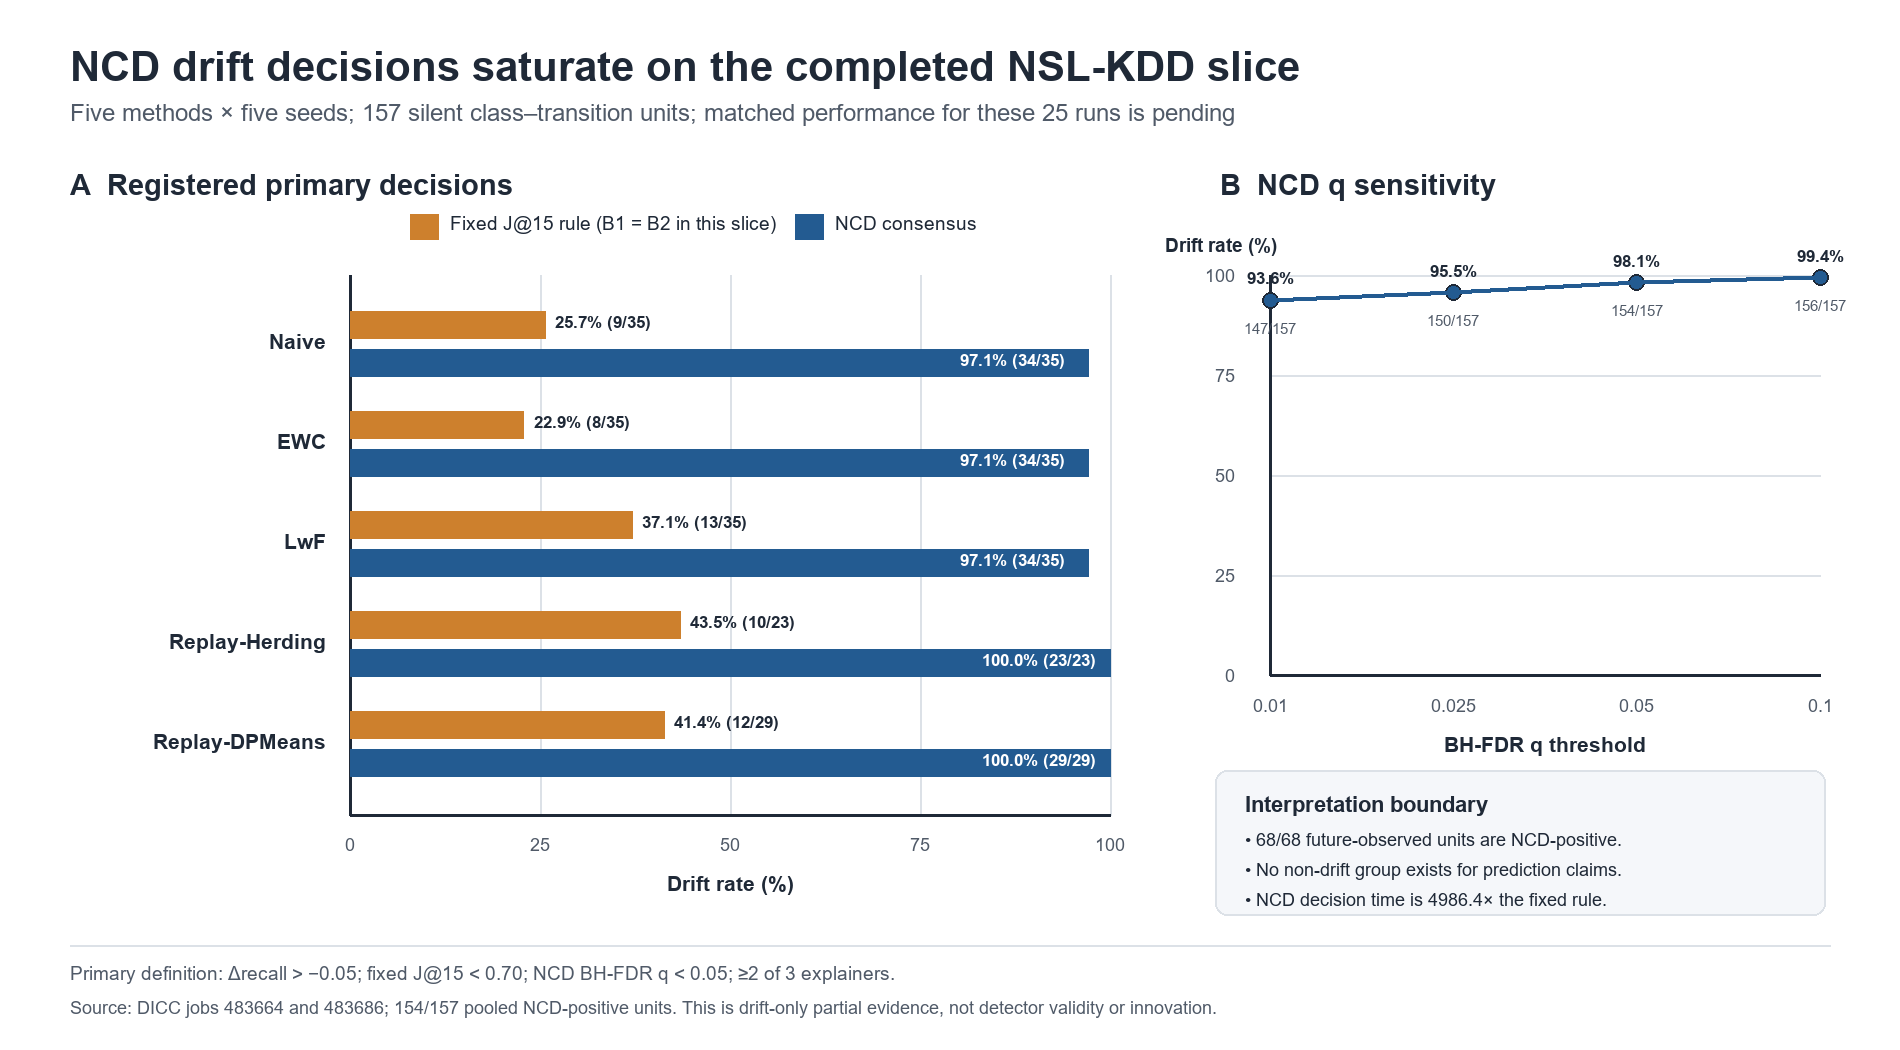
\includegraphics[width=\textwidth]{figures/nsl_25run_drift_saturation.png}
  \caption{Completed NSL-KDD drift-only evidence for five learners and five
  seeds (25 runs).  Left: the fixed B1/B2 rule and \ncd{} drift rates by
  learner.  Right: pooled \ncd{} sensitivity to the registered $q$ values.
  The near-total \ncd{} marking rate, the absence of a non-drift comparison
  group among future-observed units, and the 4986.4-fold decision-time ratio
  support a saturation diagnosis, not detector validity, incremental utility,
  substantive innovation, or governance readiness.}
  \label{fig:nsl25-saturation}
\end{figure*}

\begin{figure*}[t]
  \centering
  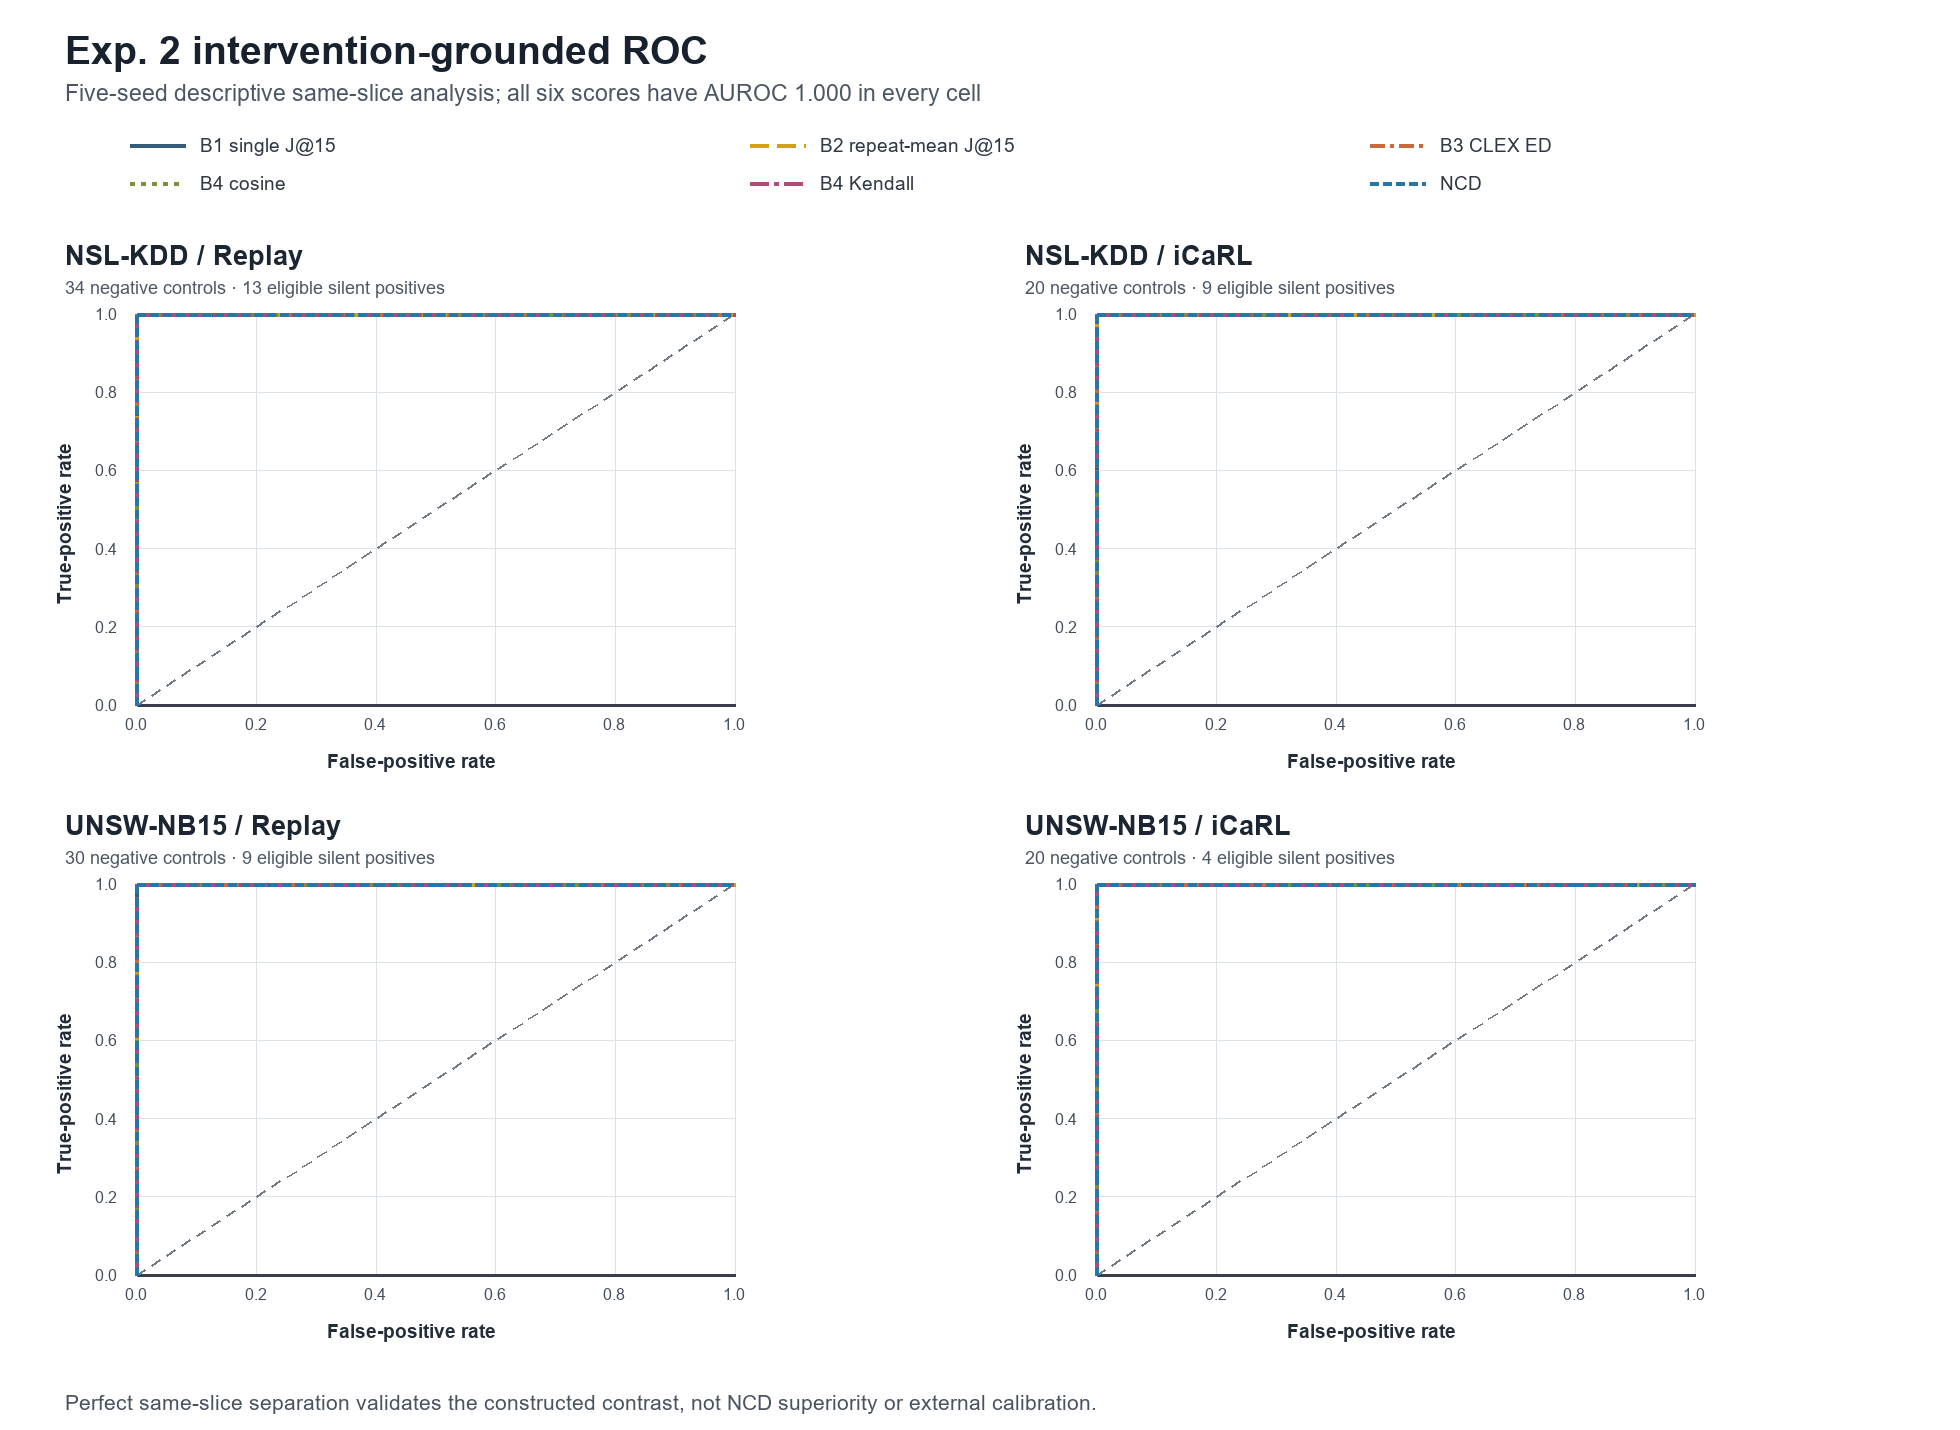
\includegraphics[width=\textwidth]{figures/exp2_four_cell_roc.png}
  \caption{Five-seed descriptive ROC curves for the four frozen Exp.~2
  dataset--learner cells.  All six continuous scores have AUROC 1.000 in every
  cell.  The curves use the same intervention constructions for selection and
  evaluation and are not externally calibrated.}
  \label{fig:exp2roc}
\end{figure*}

Removing probe bootstrap reduces eligible positive detections in all four
cells, whereas removing explainer repeats preserves every eligible positive
and removes the single UNSW-NB15 iCaRL false positive.  This ablation does not
uniquely validate the full mechanism.  The supported interpretation is that
repeated explanation measurement detects these benchmark interventions, while
the simpler repeat-mean rule is sufficient on the observed cases.

Figure~\ref{fig:exp2roc} likewise does not identify a superior detector.  The
perfect same-slice AUROC in every cell shows that the constructed eligible
positives are separable from the negative controls by all six scores.  Because
the same constructions define and evaluate this contrast, the figure supports
benchmark operability but not external discrimination, calibration, or NCD
novelty.

\section{Complete real class-incremental measurement}

Table~\ref{tab:exp3full} contains the complete registered Phase-I matrix:
four datasets, seven learners, five seeds, and 140 unique
dataset--learner--seed runs.  The fail-closed aggregation found no missing or
duplicate identity and binds each of its 12 drift/performance inputs by SHA-256.
The conditional OFRA arm in the work order is not part of this matrix: the
current NCD artifact loader consumes a single differentiable MLP checkpoint,
whereas the maintained OFRA implementation combines a frozen encoder,
per-class binary heads, and a non-differentiable router and does not emit the
same checkpoint artifact.  The older head-path SHAP pilot excludes the router
and supplies only one explainer, so it is not a conforming substitute.  This is
an explicit scope limitation, not evidence that OFRA is infeasible.  Accuracy,
balanced accuracy, macro F1, and forgetting in the table are five-seed means;
drift rates pool silent class--transition counts rather than averaging seed
percentages.

\begin{figure*}[t]
  \centering
  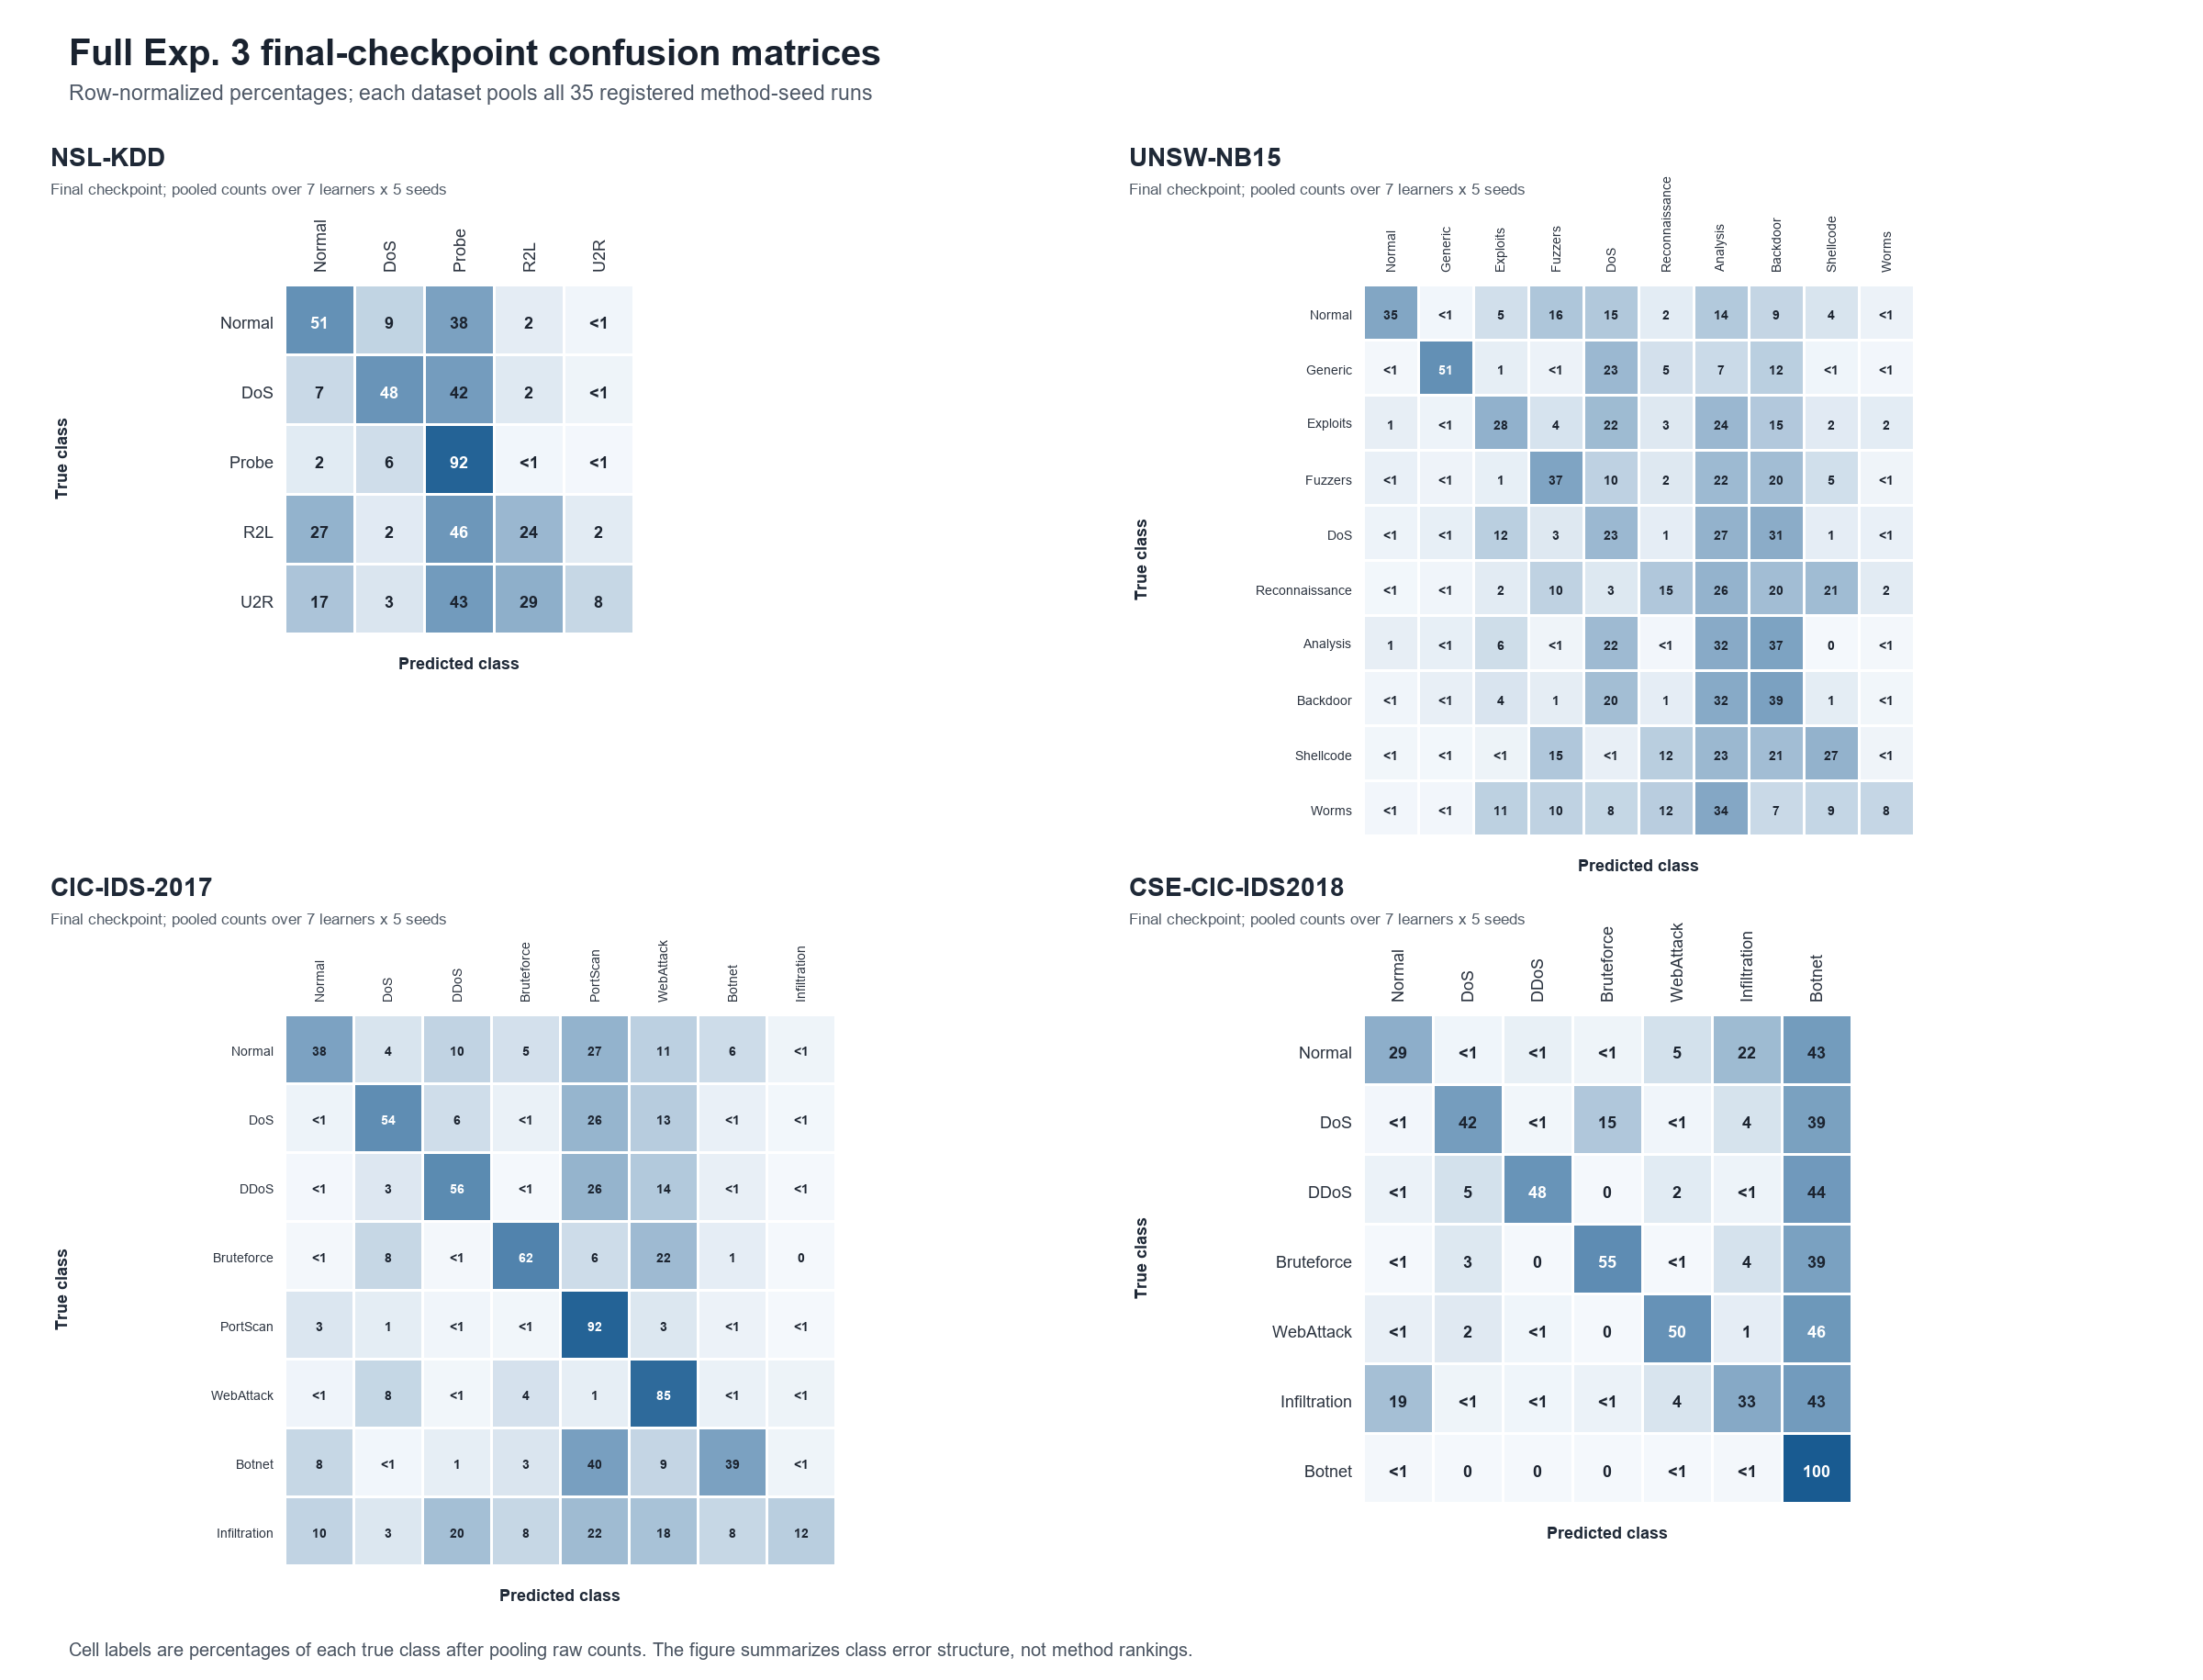
\includegraphics[width=\textwidth]{figures/full_exp3_confusion_matrices.png}
  \caption{Complete Phase-I final-checkpoint confusion matrices.  Each panel
  pools raw counts over all seven learners and five seeds for one dataset and
  then normalizes within each true class.  Pooling exposes the overall
  class-specific error structure but does not constitute a learner ranking.}
  \label{fig:full-confusion}
\end{figure*}

Figure~\ref{fig:full-confusion} provides the corresponding four-dataset
per-class view.  Pooling counts before normalization avoids giving small
true-class denominators the same weight as large ones.  It also reveals why a
single accuracy number is insufficient: rare classes such as NSL-KDD U2R and
UNSW-NB15 Worms remain broadly confused even when some replay learners have
substantially higher aggregate accuracy.

\begin{table}[p]
\centering
\caption{Complete Exp.~3 frozen-test performance and rule-defined silent-drift
rates (\%).  Performance and signed forgetting are five-seed means.  Drift
denominators are pooled silent class--transition units at the five-point recall
tolerance.  These are observational measurements, not detector-validity or
learner-superiority claims.}
\label{tab:exp3full}
\resizebox{\textwidth}{!}{%
\begin{tabular}{llrrrrrrr}
\toprule
Dataset & Learner & Acc. & BAcc. & Macro F1 & Forget. & B1 drift & B2 drift & \ncd{} drift \\
\midrule
NSL-KDD & Naive & 13.32 & 21.54 & 6.61 & 43.11 & 25.71 & 25.71 & 97.14 \\
 & EWC & 13.87 & 21.87 & 7.01 & 42.69 & 22.86 & 22.86 & 97.14 \\
 & LwF & 13.98 & 21.90 & 7.23 & 42.65 & 37.14 & 37.14 & 97.14 \\
 & Replay & 79.98 & 59.96 & 59.73 & 2.82 & 62.96 & 59.26 & 100.00 \\
 & Replay-H & 76.40 & 58.41 & 56.97 & 11.19 & 43.48 & 43.48 & 100.00 \\
 & Replay-DP & 79.97 & 57.78 & 58.62 & 3.67 & 41.38 & 41.38 & 100.00 \\
 & iCaRL & 77.54 & 70.90 & 62.68 & 6.57 & 30.30 & 30.30 & 96.97 \\
\midrule
UNSW-NB15 & Naive & 3.11 & 11.67 & 1.92 & 67.20 & 86.36 & 86.36 & 100.00 \\
 & EWC & 13.79 & 12.03 & 7.14 & 67.06 & 79.37 & 79.37 & 96.83 \\
 & LwF & 1.18 & 10.79 & 0.71 & 67.67 & 77.27 & 77.27 & 100.00 \\
 & Replay & 63.30 & 42.13 & 34.00 & 33.44 & 31.67 & 30.00 & 98.33 \\
 & Replay-H & 62.19 & 43.30 & 33.52 & 34.18 & 50.00 & 51.61 & 96.77 \\
 & Replay-DP & 60.27 & 40.79 & 30.52 & 32.68 & 38.46 & 36.92 & 96.92 \\
 & iCaRL & 51.22 & 46.06 & 28.15 & 35.45 & 18.87 & 18.87 & 98.11 \\
\midrule
CIC-IDS-2017 & Naive & 26.88 & 29.28 & 12.85 & 60.57 & 77.42 & 77.42 & 100.00 \\
 & EWC & 28.18 & 21.13 & 14.51 & 71.45 & 88.46 & 88.46 & 100.00 \\
 & LwF & 23.91 & 27.07 & 10.77 & 63.50 & 96.55 & 96.55 & 100.00 \\
 & Replay & 91.88 & 76.38 & 61.91 & 6.19 & 96.97 & 96.97 & 100.00 \\
 & Replay-H & 78.19 & 75.11 & 54.85 & 14.98 & 96.97 & 93.94 & 100.00 \\
 & Replay-DP & 88.48 & 78.45 & 60.59 & 9.12 & 93.94 & 93.94 & 100.00 \\
 & iCaRL & 69.83 & 74.36 & 46.94 & 12.38 & 84.21 & 84.21 & 100.00 \\
\midrule
CSE-CIC-IDS2018 & Naive & 19.05 & 16.38 & 6.64 & 90.92 & 88.46 & 88.46 & 100.00 \\
 & EWC & 16.66 & 14.32 & 4.15 & 93.34 & 69.23 & 69.23 & 100.00 \\
 & LwF & 16.72 & 14.38 & 4.43 & 92.35 & 84.00 & 84.00 & 100.00 \\
 & Replay & 79.82 & 82.48 & 71.60 & 13.40 & 92.50 & 92.50 & 100.00 \\
 & Replay-H & 79.84 & 82.49 & 71.46 & 13.15 & 93.33 & 93.33 & 100.00 \\
 & Replay-DP & 79.99 & 82.13 & 71.31 & 13.17 & 88.57 & 88.57 & 100.00 \\
 & iCaRL & 65.80 & 64.34 & 56.34 & 26.72 & 41.94 & 41.94 & 100.00 \\
\bottomrule
\end{tabular}%
}
\end{table}

At the primary thresholds, B1 labels 695 of 1088 silent units (63.88\%)
and B2 labels 692 (63.60\%), whereas \ncd{} labels 1076 (98.90\%).  The
dataset-level \ncd{} rates are 98.16\% for NSL-KDD, 98.16\% for UNSW-NB15,
and 100\% for each CIC dataset.  Its pooled all-explainer agreement is 98.07\%,
compared with 62.96\% for B1 and 63.14\% for B2.  Because nearly every \ncd{}
decision is positive, the high agreement is a saturation symptom rather than
evidence of discrimination.

\begin{figure*}[t]
  \centering
  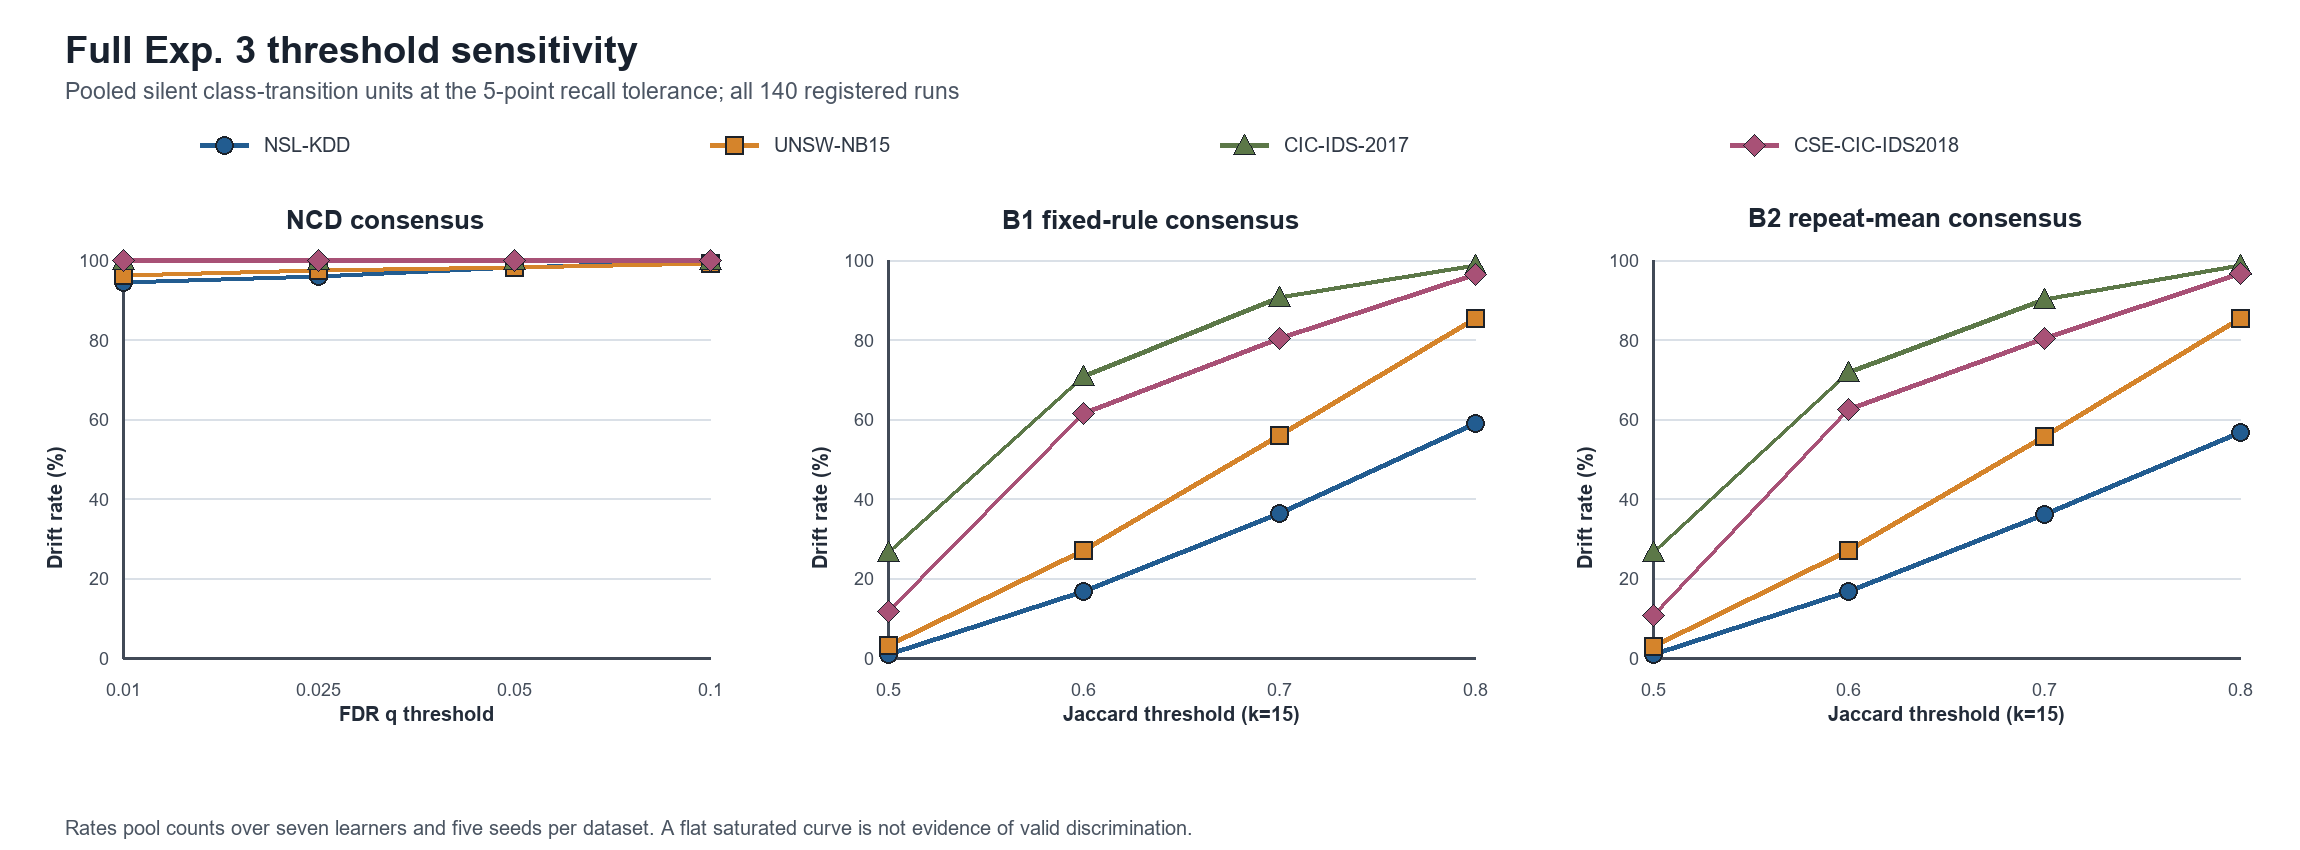
\includegraphics[width=\textwidth]{figures/full_exp3_threshold_sensitivity.png}
  \caption{Complete threshold sensitivity at the five-point silent-recall
  tolerance.  Rates pool class--transition counts over all seven learners and
  five seeds within each dataset.  B1 and B2 use cross-explainer consensus at
  $k=15$.  The near-flat \ncd{} curves remain saturated, so their stability is
  not evidence of valid calibration.}
  \label{fig:full-sensitivity}
\end{figure*}

Figure~\ref{fig:full-sensitivity} closes the registered threshold audit.  Over
$q\in\{0.01,0.025,0.05,0.10\}$, the pooled \ncd{} rate changes only from
97.33\% to 99.54\%.  B1 changes from 9.19\% to 84.93\%, and B2 from 8.92\%
to 84.56\%, over Jaccard thresholds 0.50--0.80.  Thus \ncd{} is numerically
less threshold-sensitive only because it calls nearly everything drift.

The future-recall contrast is likewise non-identifying.  Among silent units
with a later checkpoint, 415 follow an \ncd{} drift decision and only eight do
not.  Their median future recall changes are respectively $+0.00124$ and
$+0.02688$, while 96/415 and 1/8 are negative.  This extreme imbalance does
not support prediction or causality.  Recorded stage wall time totals 5610.37
seconds for training, 49882.17 seconds for explanation extraction, 0.557
seconds for the fixed decision, and 2733.26 seconds for NCD permutation.
Permutation therefore adds 5.48\% of explanation time but is 4907.49 times the
negligible fixed-rule decision time.  These are summed recorded wall times, not
hardware-normalized CPU/GPU hours.

\section{Discussion}

The main empirical result is negative but useful.  Noise calibration is
technically feasible and the intervention benchmark is auditable, yet the
current combination does not add identifiable decision value over repeat
averaging.  Exp.~2 ties B2 on every eligible positive endpoint and incurs one
additional false positive.  The complete Exp.~3 matrix then labels 98.90\% of
silent units as drift, including every eligible unit in both CIC datasets.
Together these results argue against promoting \ncd{} as the project's
substantive innovation or using its observed rate as the prevalence of true
silent dependency change.

A post-hoc effect-size diagnostic tests whether a simple gate can rescue this
saturation without losing intervention sensitivity.  For each explainer, the
noise gate is the 95th percentile of the Exp.~2 N1/N2 effect distribution;
the stronger positive-anchor gate is the larger of that value and the lower
5th-percentile eligible-positive effect.  Table~\ref{tab:saturation-diagnostic}
reports four-cell holdout evaluation in Exp.~2 and application to the frozen
Exp.~3 silent units.  The noise gate removes the sole negative-control false
positive while retaining 34/34 eligible positives, but leaves 98.90\% or
98.25\% of Exp.~3 units positive.  The positive-anchor variants reduce the
rate to about 63.4\%, but detect only 29/34 held-out positives and therefore
fail the requirement to match B2 sensitivity.  Moreover, 5351/5565 (96.15\%)
Exp.~3 explainer-level tests attain the minimum permutation $p$-value
$1/1001$.  These exploratory results reject a threshold-only rescue; they do
not validate a replacement detector.

\begin{table}[t]
\centering
\caption{Exploratory saturation diagnostic.  Exp.~2 counts are summed over
four dataset--learner cell holdouts; Exp.~3 counts use the 1088 frozen silent
units.  N95 denotes a negative-control 95th-percentile effect gate and P5 the
stronger positive-anchor gate.  Abs and rel use absolute effect and effect
relative to within-checkpoint variation, respectively.}
\label{tab:saturation-diagnostic}
\begin{tabular}{@{}lrrr@{}}
\toprule
Rule & Exp.~2 neg. FP & Exp.~2 pos. & Exp.~3 positive \\
\midrule
B2 repeat mean & 0/104 & 34/34 & 692/1088 (63.60\%) \\
Current \ncd{} & 1/104 & 34/34 & 1076/1088 (98.90\%) \\
\ncd{} + N95 abs & 0/104 & 34/34 & 1076/1088 (98.90\%) \\
\ncd{} + N95 rel & 0/104 & 34/34 & 1069/1088 (98.25\%) \\
\ncd{} + P5 abs & 0/104 & 29/34 & 690/1088 (63.42\%) \\
\ncd{} + P5 rel & 0/104 & 29/34 & 693/1088 (63.69\%) \\
\bottomrule
\end{tabular}
\end{table}

This does not erase RQ1.  It narrows the next scientific question from
``can estimator noise be calibrated?'' to ``which explanation or aggregation
rule tracks intervention-confirmed dependency change without saturation?''
Any replacement mechanism must keep matched data roles, seeds, thresholds,
resource accounting, and B2 as a mandatory control.  A metric bundle,
threshold adjustment, or additional classifier alone would not satisfy that
requirement.

RQ3 also remains open.  A governance layer may record evidence without
suppressing alerts, but no current result shows that the drift evidence is
faithful enough to drive admission, suspension, escalation, refusal, or
recertification.  Governance evaluation must therefore remain downstream of
detector validity and must prove binary decision invariance.

\section{Limitations}

The intervention benchmark is constructed and uses the same public datasets
as evaluation; it is not an independent deployment study.  Some P2 cells have
no eligible construction, and no Exp.~3 run uses an independent calibration
split.  The complete 140-run Phase-I matrix excludes the work order's
conditional OFRA arm; no conforming OFRA NCD run is claimed.  The pooled
confusion matrices intentionally combine heterogeneous learners and therefore
describe class error structure rather than comparative learner performance.
Recorded stage times are wall-clock measurements rather than
utilization-weighted CPU/GPU hours.  Silent drift is operationalized through a
recall tolerance and remains sensitive to probe population, explainer,
distance, and aggregation choices.  NCD significance is not equivalent to
causal dependency change.  No current result establishes substantive
innovation, cross-domain generality, publication acceptance, or a validated
governance mechanism.  The effect-size gates in
Table~\ref{tab:saturation-diagnostic} were selected post hoc from Exp.~2 and
require a fresh frozen intervention set before any confirmatory use.

\section{Conclusion}

An explanation-drift study becomes scientifically interpretable only when it
separates estimator variability from model change and evaluates the resulting
decision against known dependency changes.  On the completed intervention
matrix, repeated explanations work, but the proposed permutation/FDR decision
does not improve on repeat averaging.  On the complete registered Phase-I
matrix, the same decision labels 1076 of 1088 silent units as drift and offers
no balanced comparison for subsequent recall.  The honest conclusion is
therefore a bounded measurement result and a rejected superiority claim.  RQ1
remains scientifically open until a mechanism demonstrates selective,
intervention-grounded incremental value; RQ3 remains downstream of that
validity result.

\begin{thebibliography}{10}
\bibitem{cossu2024clex}
A.~Cossu, F.~Spinnato, R.~Guidotti, and D.~Bacciu.
\newblock Drifting explanations in continual learning.
\newblock \emph{Neurocomputing}, 597:127960, 2024.
\newblock \url{https://doi.org/10.1016/j.neucom.2024.127960}.

\bibitem{ebrahimi2021rrr}
S.~Ebrahimi et al.
\newblock Remembering for the right reasons: Explanations reduce catastrophic forgetting.
\newblock \emph{Applied AI Letters}, 2(4):e44, 2021.
\newblock \url{https://doi.org/10.1002/ail2.44}.

\bibitem{nugraha2026e2d2}
B.~Nugraha and T.~Bauschert.
\newblock E2D2: A modular framework for explanation-based drift detection in unsupervised network intrusion detection.
\newblock \emph{IFIP Networking}, 2026.
\newblock \url{https://doi.org/10.23919/IFIPNetworking70592.2026.11578962}.

\bibitem{lamaakal2026drift2act}
I.~Lamaakal, C.~Yahyati, K.~El~Makkaoui, I.~Ouahbi, and Y.~Maleh.
\newblock Drift-to-action controllers: Budgeted interventions with online risk certificates.
\newblock arXiv:2603.08578, 2026.

\bibitem{covert2021kernel}
I.~Covert and S.-I. Lee.
\newblock Improving KernelSHAP: Practical Shapley value estimation using linear regression.
\newblock In \emph{AISTATS}, pages 3457--3465, 2021.

\bibitem{hill2024gpec}
D.~Hill, A.~Masoomi, M.~Torop, S.~Ghimire, and J.~Dy.
\newblock Boundary-aware uncertainty for feature attribution explainers.
\newblock In \emph{AISTATS}, pages 55--63, 2024.

\bibitem{williamson2020spvim}
B.~Williamson and J.~Feng.
\newblock Efficient nonparametric statistical inference on population feature importance using Shapley values.
\newblock In \emph{ICML}, pages 10282--10291, 2020.

\bibitem{hwang2026multiplicity}
H.~Hwang, S.~Lee, L.~Rosenblatt, J.~Stoyanovich, and S.~E. Whang.
\newblock Explanation multiplicity in SHAP: Characterization and assessment.
\newblock arXiv:2601.12654, 2026.
\end{thebibliography}

\end{document}
